\begin{center}
\footnotesize\noindent\fbox{
	\parbox{\textwidth}{
	 Ripetere una procedura analoiga a quella del precedente esercizio utilizzando il metodo di Gauss-Seidel.
}
}\end{center}


\begin{center}
	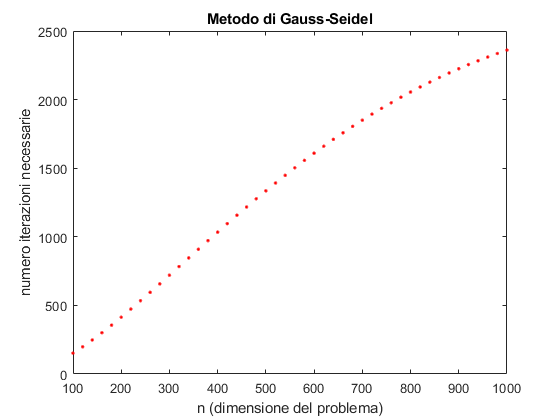
\includegraphics[scale=0.9]{cap6/6_4.png}
\end{center}

\noindent Il codice Matlab utilizzato per realizzarle il grafico mostrato \'e il seguente: \\

\lstinputlisting[language=Matlab]{cap6/6_4.m}
